\section*{Addendum - Building the morphisms $S_G, T_G, S_{m,n}, T_{m,n}$}
%
%
In Section~\ref{sec: turning executions into circuits} we mentioned 
a couple of boolean circuits, $S_G, T_G : \Bool^E \to \Bool^V$: 
They depend on a fixed graph $G$, and return 
as output the enumeration of a source and target vertex, respectively, 
of an edge whose enumeration is specified as input.

The beauty of category theory lies precisely in the possibility
 to abstract from the definition of $S_G$ and $T_G$, just focusing 
on how these functions had to be used to assemble the whole verifying 
circuit for $G$. Nevertheless, a precise
description of these circuits is still needed to make an implementation
possible, which we are going to provide in this addendum. We warn the reader 
that our solution is far from being optimal in terms of complexity, so it should be 
understood as a proof of concept.

In the following, we will explain the process for the circuit $S_G$, 
the one for $T_G$ being similar. First, we realize $S_G$ as a table using the incidency 
matrix of the graph $G$:
%
%
\begin{center}\scriptsize
  \begin{tabular}{c|c}
    Edge & Source Vertex\\
  \hline
    $\Id{v_1}$   & $v_1$\\
    \dots              & \dots \\
    $\Id{v_n}$   & $v_n$ \\
    $e_1$           & $s(e_1)$ \\
    \dots             & \dots \\
    $e_m$          & $s(e_m)$\\
    $u_1$           & $\Zero$ \\
    \dots             & \dots \\
    $u_k$           & $\Zero$\\
  \end{tabular}
\end{center}
%
Here $s(\_)$ represents the source function associated to $G$.
From here, we switch to enumerations, where we denote 
with $x^i_j$ the $i$-th binary digit of the enumeration of 
element $x_j$:
%
%
\begin{center}\scriptsize
  \begin{tabular}{ccc|ccc}
    Edge 1st bit & & Edge $E$-th bit & Source 1st bit && Source $V$-th bit\\
  \hline
    $\Id{v_1}^1$ & $\dots$ & $\Id{v_1}^E$ & $v_1^1$       & $\dots$ & $v_1^V$\\
                           & $\dots$ &                         &                      & $\dots$ & \\
    $\Id{v_n}^1$ & $\dots$ & $\Id{v_n}^E$ & $v_n^1$       & $\dots$ & $v_n^V$\\
    $e_1^1$          & $\dots$ & $e_1^E$         & $s(e_1)^1$   & $\dots$ & $s(e_1)^V$\\
                            & $\dots$ &                        &                      & $\dots$ & \\
    $e_m^1$         & $\dots$ & $e_m^E$        & $s(e_m)^1$  & $\dots$ & $s(e_m)^V$\\
    $u_1^1$          & $\dots$ & $u_1^E$         & $0$               & $\dots$ & $0$\\
                            & $\dots$ &                        &                      & $\dots$ & \\
    $u_k^1$          & $\dots$ & $u_k^E$         & $0$               & $\dots$ & $0$\\
  \end{tabular}
\end{center}
%
We now split the table into $V$ different tables, each returning only one digit of the 
vertex enumeration:
%
%
\begin{center}\scriptsize
  \begin{tabular}{ccc|c}
    Edge 1st bit & & Edge $E$-th bit & Source 1st bit \\
  \hline
    $\Id{v_1}^1$ & $\dots$ & $\Id{v_1}^E$ & $v_1^1$\\
                           & $\dots$ &                         &\\
    $\Id{v_n}^1$ & $\dots$ & $\Id{v_n}^E$ & $v_n^1$\\
    $e_1^1$          & $\dots$ & $e_1^E$         & $s(e_1)^1$\\
                            & $\dots$ &                        &\\
    $e_m^1$         & $\dots$ & $e_m^E$        & $s(e_m)^1$\\
    $u_1^1$          & $\dots$ & $u_1^E$         & $0$\\
                            & $\dots$ &                        &\\
    $u_k^1$          & $\dots$ & $u_k^E$         & $0$\\
  \end{tabular}
  \hspace{1em}
    $\dots$
  \hspace{1em}
  \begin{tabular}{ccc|c}
    Edge 1st bit & & Edge $E$-th bit & Source $V$-th bit \\
  \hline
    $\Id{v_1}^1$ & $\dots$ & $\Id{v_1}^E$ & $v_1^V$\\
                           & $\dots$ &                         &\\
    $\Id{v_n}^1$ & $\dots$ & $\Id{v_n}^E$ & $v_n^V$\\
    $e_1^1$          & $\dots$ & $e_1^E$         & $s(e_1)^V$\\
                            & $\dots$ &                        &\\
    $e_m^1$         & $\dots$ & $e_m^E$        & $s(e_m)^V$\\
    $u_1^1$          & $\dots$ & $u_1^E$         & $0$\\
                            & $\dots$ &                        &\\
    $u_k^1$          & $\dots$ & $u_k^E$         & $0$\\
  \end{tabular}
\end{center}
%
Using standard techniques~\cite{Vollmer1999} we are able to turn each one of 
these tables into a circuit. We then obtain a bunch 
of morphisms in $\Bcirc$:
%
%
\begin{equation*}
  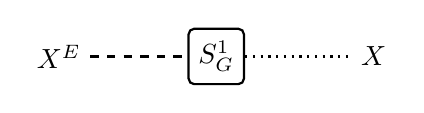
\begin{tikzpicture}[baseline=0pt]
    \node[draw, minimum height=20, minimum width=20, rounded corners=2, thick] (S) at (0,0) {$S_G^1$};

    \node (Xe) at (-2,0) {$X^E$};
    \node (Xv) at (2,0) {$X$};

    \draw[-, dashed,thick] (Xe) to (S.west);
    \draw[-, dotted, thick] (S.east) to (Xv);
  \end{tikzpicture}
  \qquad \dots \qquad
  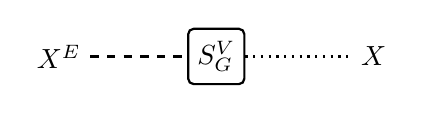
\begin{tikzpicture}[baseline=-1pt]
    \node[draw, minimum height=20, minimum width=20, rounded corners=2, thick] (S) at (0,0) {$S_G^V$};

    \node (Xe) at (-2,0) {$X^E$};
    \node (Xv) at (2,0) {$X$};

    \draw[-, dashed, thick] (Xe) to (S.west);
    \draw[-, dotted, thick] (S.east) to (Xv);
  \end{tikzpicture}
\end{equation*}
% 
The resulting morphism $S_G$ is obtained by just copying the 
input and tensoring the morphisms together:
%
%
\begin{equation*}
  \begin{tikzpicture}
    \node at (4.25,0) {};
    \node[draw, minimum height=20, minimum width=20, rounded corners=2, thick] (SV) at (0,-1) {$S_G^V$};
    \node[thick] (Sdots) at (0,0.15)  {$\vdots$};
    \node[draw, minimum height=20, minimum width=20, rounded corners=2, thick] (S1) at (0,1)  {$S_G^1$};
    \node[draw, circle, radius=5pt, thick] (copy) at (-2,0) {};

    \node (XeV) at (-4,0) {$X^E$};

    \node (XvV) at (2,-1) {$X$};
    \node (Xv1) at (2,1) {$X$};

    \draw[-, dashed, thick] (XeV) to (copy.west);
    \draw[bend left, dashed, thick] (copy.north) to (S1.west);
    \draw[bend right, dashed, thick] (copy.south) to (SV.west);

    \draw[-, dotted, thick] (SV.east) to (XvV);
    \draw[-, dotted, thick] (S1.east) to (Xv1);
  \end{tikzpicture}
\end{equation*}
%
Here one should note that the $V$-fold monoidal product of $X$ is 
just $X^V$, so the string diagram above is a morphism of the right type, from 
$X^E$ to $X^V$.

Now we focus on the circuits $S_{m,n}, T_{m,n}: X^{f(m,n)} \otimes X^m \to X^n $.
These accept a graph enumeration of $f(m,n)$ bits in input, along with an edge 
enumeration of $m$ bits, and return a vertex enumeration of $n$ bits, representing the 
source and target, respectively, of the edge provided in the specified graph.

Again, we focus on $S_{m,n}$, the procedure for $T_{m,n}$ being
similar. We start by noticing that for a fixed
bitstring $s$ of length $f(m,n)$, we can produce a circuit 
$F_s: X^{f(m,n)} \to X$ (called \emph{filter for $s$}) that outputs $1$ only 
if the input is $s$, and $0$ otherwise: For each digit composing 
$s$, we concatenate it with a $\NOT$ gate if it is $0$, and we leave it as it is 
otherwise. Then we wire all the bits with $\AND$ ports. For instance, 
the circuit below, working for inputs of $4$ bits, 
outputs $1$ only if the input is $1001$.
%
%
\begin{center}
  \resizebox{6cm}{2.5cm}{
  \begin{circuitikz}
    \draw (-1,-0.14)  node[american not port, scale = 0.3] (a1){};
    \draw (-1,1.14)  node[american not port, scale = 0.3] (a2){};
    \draw (0,0)  node[american and port, scale = 0.5] (b1){};
    \draw (0,1) node[american and port, scale = 0.5] (b2){};
    \draw (1,0.5)  node[american and port, scale = 0.5] (c1){};

    \draw[-] (b1.out) |- (c1.in 2);
    \draw[-] (b2.out) |- (c1.in 1);
    \draw[-] (a2.out) |- (b2.in 1);
    \draw[-] (a1.out) |- (b1.in 2);

    \draw[-] (a1.in) -- +(-1.5,0);
    \draw[-] (a2.in) -- +(-1.5,0);
    \draw[-] (b1.in 1) -- +(-2,0);
    \draw[-] (b2.in 2) -- +(-2,0);

    \draw[-] (c1.out) -- +(1.5,0);
  \end{circuitikz}}
\end{center}
%
Interpreting a bitstring $s$ as the enumeration of a 
graph $G$ with $m$ edges and $n$ vertexes, we can consider the circuit:
%
%
\begin{equation*}
  \begin{tikzpicture}
    \node at (4.25,0) {};
    \node[draw, minimum height=20, minimum width=20, rounded corners=2, thick] (SG) at (0,0) {$S_G$};
    \node[draw, minimum height=20, minimum width=20, rounded corners=2, thick] (F) at (0,1)  {$F_s$};
    \node[draw, circle, radius=5pt, thick] (copy) at (1,1) {};
    \draw (3,0)  node[american and port, scale = 0.5] (a2){};
    \draw (3,1)  node[american and port, scale = 0.5] (a1){};

    \node (XeV) at (-2,0) {$X^m$};
    \node (XF) at (-2,1) {$X^{f(m,n)}$};
    \node (XOut1) at (4.5,1) {$X$};
    \node (XOut2) at (4.5,0) {$X$};

    \node (XSG1) at (0.6,-0.45) {$X$};
    \node (XSGDots) at (1,0.2) {\tiny{$\vdots$}};
    \node (AndDots) at (2.9,0.6) {\scriptsize{$\vdots$}};
    \node (XSG2) at (0.6,0.45) {$X$};
    \node (XF1) at (0.5,1.25) {$X$};
  
    \draw[-, dashed, thick] (SG.west) to (XeV);
    \draw[-, densely dotted, thick] (F.west) to (XF);

    \draw[-, dotted, thick] (F.east) to (copy.west);

    \draw[-, out=25, in=180, dotted, thick] (copy.north) to (a1.in 1);
    \draw[-, out=-25, in=180, dotted, thick] (copy.south) to (a2.in 1);

    \draw[-, out=15, in=200, dotted, thick] ([yshift=5pt]SG.east) to (a1.in 2);
    \draw[-, out=0, in=180, dotted, thick] ([yshift=-5pt]SG.east) to (a2.in 2);

    \draw[-, dotted, thick] (a1.out) to (XOut1.west);
    \draw[-, dotted, thick] (a2.out) to (XOut2.west);
  \end{tikzpicture}
\end{equation*}
%
That is, we are connecting the output of $F_s$ with each output bit of 
$S_G$ using $\AND$ ports. The result is a circuits 
$S_{m,n}^G: X^{f(m,n)} \otimes X^m \to X^n$ that reduces to $S_G$
when the input on $X^{f(n,m)}$ is the enumeration of the graph $G$, 
while it reduces to the constant $0$ circuit in any other case.

The circuit $S_{m,n}$ is obtained by tensoring together all the 
$S_{m,n}^G$ gates for each graph $G$ of $m$ edges and $v$ vertexes,
by copying the inputs and taking the $\OR$ of the outputs.
%
%
\begin{equation*}
  \begin{tikzpicture}
    \node at (4.25,0) {};
    \node[draw, minimum height=20, minimum width=40, rounded corners=2, thick] (SV) at (0,-1) {$S_{m,n}^{G_{f(m,n)}}$};
    \node[thick] (Sdots) at (0,0.15)  {$\vdots$};
    \node[draw, minimum height=20, minimum width=40, rounded corners=2, thick] (S1) at (0,1)  {$S_{m,n}^{G_1}$};
    \node[draw, circle, radius=5pt, thick] (copyGraph) at (-2,1) {};
    \node[draw, circle, radius=5pt, thick] (copyEdge) at (-2,-1) {};
    \draw (2.5,-1.15)  node[american or port, scale = 0.5] (o2){};
    \draw (2.5,1.15)  node[american or port, scale = 0.5] (o1){};

    \node (Xg) at (-4,1) {$X^{f(m,n)}$};
    \node (Xe) at (-4,-1) {$X^m$};

    \node[thick] (Sdots) at (0,0.15)  {$\vdots$};
    \node[thick] (Ordots) at (2.25,0.15)  {$\vdots$};
    \node (FirstDots) at (0.85,1.1) {\tiny{$\vdots$}};
    \node (SecondDots) at (0.85,-0.9) {\tiny{$\vdots$}};


    \node (XvV) at (4,-1.15) {$X$};
    \node (Xv1) at (4,1.15) {$X$};

    \draw[-, densely dotted, thick] (Xg) to (copyGraph.west);
    \draw[-, dashed, thick] (Xe) to (copyEdge.west);

    \draw[-, in=180, out=45, densely dotted, thick] (copyGraph.north) to ([yshift=5pt]S1.west);
    \draw[-, in=180, out=-45, densely dotted, thick] (copyGraph.south) to ([yshift=5pt]SV.west);
    \draw[-, in=180, out=45, dashed, thick] (copyEdge.north) to ([yshift=-5pt]S1.west);
    \draw[-, in=180, out=-45, dashed, thick] (copyEdge.south) to ([yshift=-5pt]SV.west);

    \draw[-, in=180, out=20, dotted, thick] ([yshift=5pt]SV.east) to (o1.in 2);
    \draw[-, in=180, out=-20, dotted, thick] ([yshift=-5pt]SV.east) to (o2.in 2);

    \draw[-, in=180, out=20, dotted, thick] ([yshift=5pt]S1.east) to (o1.in 1);
    \draw[-, in=180, out=-20, dotted, thick] ([yshift=-5pt]S1.east) to (o2.in 1);

    \draw[-, densely dotted, thick] (o1.out) to (Xv1.west);
    \draw[-, densely dotted, thick] (o2.out) to (XvV.west);
  \end{tikzpicture}
\end{equation*}
%
Feeding the enumeration of a graph $G$ to the circuit above has the following effect:
Exactly one of the tensored circuits will reduce to $S_G$, while
all the others will reduce to the constant $0$ circuit. Since $0$ is a unit for $\OR$, 
the resulting circuit reduces to $S_G$.